\section{连续时间的随机路径}
\label{sec:ctsp-paths}

第~\ref{chap:stochastic-processes-and-sample-paths}章把随机过程写成共同概率空间上的随机变量族$(X_t)_{t\in\mathbb T}$，并区分了固定时刻的随机变量与固定实现的样本路径。本节把索引集取为$\mathbb T=[0,\infty)$。我们先构造两个可以直接计算的模型：按事件跳跃的Poisson过程，以及处处连续却处处抖动的Brownian运动；再回头处理不可数时刻带来的问题，即路径版本、信息结构和停时需要满足哪些额外条件。这些条件不是为抽象而抽象，后面每一个结论在使用它们时都会指出它们承担的作用。

\subsection{事件到达与Poisson过程}
\label{sec:ctsp-poisson}

\paragraph{从等待时间到计数路径}
想象一台服务器，请求一个接一个地到来。最简单的模型只规定相邻请求之间的等待时间：它们相互独立，都服从速率为$\lambda>0$的指数分布。指数分布的特点是无记忆：已经等了$s$个单位时间而请求仍未到来，再等至少$u$的概率仍是
\[
  \mathbb P(E>s+u\mid E>s)=\frac{e^{-\lambda(s+u)}}{e^{-\lambda s}}=e^{-\lambda u}=\mathbb P(E>u).
\]
因此服务器“已经空闲了多久”不提供任何关于下一次到达的信息，这正是“事件以恒定速率随机发生”的数学表达。

设$E_1,E_2,\ldots$独立同分布于$\operatorname{Exp}(\lambda)$。第$k$次到达时刻和到时刻$t$为止的到达次数分别为
\begin{equation}
  T_k=E_1+\cdots+E_k,\qquad
  N_t=\#\{k\geq1:T_k\leq t\}.
  \label{eq:ctsp-poisson-construction}
\end{equation}
同一个随机机制因此有三种描述：等待时间序列、到达时刻序列和计数路径。图~\ref{fig:ctsp-poisson-three-views}把它们画在同一条时间轴上。读者可以沿竖直方向对照：每段等待结束的地方就是一个到达时刻，计数路径恰好在那里向上跳一格，其余时间保持水平。

\begin{figure}[htbp]
  \centering
  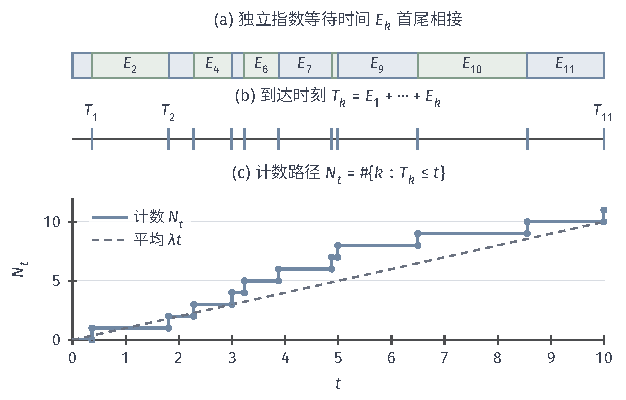
\includegraphics[width=105mm]{figures/03-optimization-evolution-and-signals/02-processes-and-trajectory-evolution/tikz/ctsp-poisson-three-views/figure.pdf}
  \caption{同一Poisson机制的三种描述（固定随机种子的一次实现，$\lambda=1$，时段$[0,10]$）。(a)独立指数等待时间首尾相接，蓝绿交替只为区分相邻段；(b)每段末端是一个到达时刻；(c)计数路径在到达时刻跳高一格，实心点是跳后的取值，空心点是跳前的左极限，虚线是平均计数$\lambda t$。}
  \label{fig:ctsp-poisson-three-views}
\end{figure}

计数路径有几条一眼可见的性质：$N_0=0$，路径非减、取非负整数、每次跳跃的高度为一，并且在每个跳跃时刻取跳后的值，即右连续；在每个时刻左侧都有极限$N_{t-}=\lim_{s\uparrow t}N_s$，跳跃量记为$\Delta N_t=N_t-N_{t-}$。另一条性质需要论证：有限时段内只有有限次跳跃。由强大数律，$T_k/k\to1/\lambda$几乎必然，所以$T_k\to\infty$，任意有界区间$[0,t]$只包含有限个到达时刻。没有这条性质，计数在有限时间内就可能变成无穷。

\paragraph{计数的Poisson规律}
从等待时间出发，可以算出固定时刻计数的分布。$T_k$是$k$个独立指数变量之和，服从$\operatorname{Gamma}(k,\lambda)$，密度为$f_k(s)=\lambda^ks^{k-1}e^{-\lambda s}/(k-1)!$。由于$\{N_t\geq k\}=\{T_k\leq t\}$，
\[
  \mathbb P(N_t=k)=\mathbb P(T_k\leq t)-\mathbb P(T_{k+1}\leq t)
  =\int_0^t[f_k(s)-f_{k+1}(s)]\,\mathrm ds .
\]
直接求导可验证$\frac{\mathrm d}{\mathrm ds}\bigl[e^{-\lambda s}(\lambda s)^k/k!\bigr]=f_k(s)-f_{k+1}(s)$，于是
\begin{equation}
  \mathbb P(N_t=k)=e^{-\lambda t}\frac{(\lambda t)^k}{k!},\qquad k=0,1,2,\ldots
  \label{eq:ctsp-poisson-marginal}
\end{equation}
即$N_t\sim\operatorname{Poisson}(\lambda t)$。$k=0$时它就是$\mathbb P(E_1>t)=e^{-\lambda t}$。

单个时刻的分布还不足以描述过程，需要知道不同时间段的计数怎样联合。无记忆性在这里起关键作用。固定$s$，在事件$\{N_s=k\}$上，已经发生的到达是$T_1,\ldots,T_k$，下一次到达的剩余等待$T_{k+1}-s$满足
\[
  \mathbb P(T_{k+1}-s>u\mid T_1,\ldots,T_k,\ N_s=k)=e^{-\lambda u},
\]
因为它是$E_{k+1}$在已知$E_{k+1}>s-T_k$条件下超出部分的分布；其后的$E_{k+2},E_{k+3},\ldots$又与过去无关。所以从时刻$s$重新计时，未来的等待时间仍是一列独立的$\operatorname{Exp}(\lambda)$变量，并且独立于$s$以前的记录。

\begin{theorem}[Poisson过程的增量]
  \label{thm:ctsp-poisson-increments}
  由式~\eqref{eq:ctsp-poisson-construction}构造的计数过程，对任意$0\leq s<t$，增量$N_t-N_s$独立于$\sigma(N_u:u\leq s)$，并服从$\operatorname{Poisson}(\lambda(t-s))$。因而对任意$0\leq t_0<t_1<\cdots<t_n$，各段增量相互独立。
\end{theorem}

\begin{proof}
上面的论证说明，$(N_{s+u}-N_s)_{u\geq0}$由一列与过去独立的$\operatorname{Exp}(\lambda)$等待时间按同样的规则生成，因此它与$(N_u)_{u\geq0}$同分布且独立于$\sigma(N_u:u\leq s)$。取$u=t-s$并用式~\eqref{eq:ctsp-poisson-marginal}得到增量分布。对多个时间段，从最后一段开始依次使用这一独立性，即得各段增量相互独立。把无记忆性写成严格的条件分布等式需要对$k$和$T_1,\ldots,T_k$的取值积分，细节见Kallenberg的概率论教材。
\end{proof}

条件分布形式的细节可参考文献\scite{math-kallenberg2021probability}。

这一定理把构造得到的对象与通常的公理式定义连接起来。以后研究随机积分时，还要允许滤过比计数自身的历史更大，因此我们按下面的形式使用Poisson过程。

\begin{definition}[Poisson过程]
  \label{def:ctsp-poisson-process}
  给定速率$\lambda>0$和滤过$(\mathcal F_t)_{t\geq0}$，适应的计数过程$N$称为相对于该滤过的\term{Poisson过程}（Poisson process），若$N_0=0$，路径右连续、非减、取整数值且每次跳跃高度为一，并且对$0\leq s<t$，$N_t-N_s$独立于$\mathcal F_s$，服从$\operatorname{Poisson}(\lambda(t-s))$。
\end{definition}

速率$\lambda$描述单位时间内的平均事件数，即$\mathbb EN_t=\lambda t$；它不是概率。从式~\eqref{eq:ctsp-poisson-marginal}在$h\downarrow0$时展开，
\[
  \mathbb P(N_{t+h}-N_t=1)=\lambda h+O(h^2),\qquad
  \mathbb P(N_{t+h}-N_t\geq2)=O(h^2).
\]
只有在短时间$h$内，$\lambda h$才近似为发生一次事件的概率。例如每分钟平均三个请求时，一分钟内至少来一个请求的概率是$1-e^{-3}\approx0.95$，而不是$3$；把$\lambda$直接当成“每步转移概率”的离散化，在$\lambda h$不小时会产生明显偏差。

\paragraph{复合Poisson过程与逐事件模拟}
很多应用中，事件的影响不是固定的一格。保险公司每收到一笔理赔，金额是随机的；股票价格在消息到达时跳变，跳幅可正可负。设$J_1,J_2,\ldots$独立同分布，并独立于计数过程$N$，定义
\begin{equation}
  C_t=\sum_{k=1}^{N_t}J_k ,
  \label{eq:ctsp-compound-poisson}
\end{equation}
称为\term{复合Poisson过程}（compound Poisson process）。它的路径仍在到达时刻跳跃，只是跳幅由标记$J_k$给出，见图~\ref{fig:ctsp-compound-poisson}。

\begin{figure}[htbp]
  \centering
  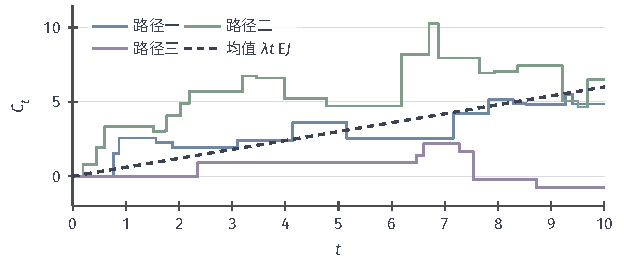
\includegraphics[width=105mm]{figures/03-optimization-evolution-and-signals/02-processes-and-trajectory-evolution/tikz/ctsp-compound-poisson/figure.pdf}
  \caption{复合Poisson过程的三条独立路径。到达速率$\lambda=1.5$，跳幅$J_k\sim\mathcal N(0.4,1)$，固定随机种子。路径在到达之间保持水平，跳幅可正可负；虚线为均值$\lambda t\,\mathbb EJ=0.6t$。单条路径可以长时间偏离均值线，均值只描述大量路径的平均。}
  \label{fig:ctsp-compound-poisson}
\end{figure}

先给定$N_t$再求平均，可以得到均值和方差。给定$N_t=n$时，$C_t$是$n$个独立标记之和，因而
\[
  \mathbb E[C_t\mid N_t]=N_t\,\mathbb EJ_1,\qquad
  \operatorname{Var}(C_t\mid N_t)=N_t\operatorname{Var}(J_1).
\]
由全期望公式与全方差公式，在$\mathbb EJ_1^2<\infty$时，
\begin{equation}
  \mathbb EC_t=\lambda t\,\mathbb EJ_1,\qquad
  \operatorname{Var}(C_t)=\lambda t\operatorname{Var}(J_1)+(\mathbb EJ_1)^2\operatorname{Var}(N_t)=\lambda t\,\mathbb EJ_1^2 .
  \label{eq:ctsp-compound-moments}
\end{equation}
方差中出现的是二阶矩$\mathbb EJ_1^2$而不是$\operatorname{Var}(J_1)$，多出的部分来自事件个数本身的随机性。

\begin{example}[十天的理赔总额]
  \label{ex:ctsp-claims}
  理赔以每天$\lambda=2$笔的速率到达，每笔金额的均值为$3$、二阶矩为$13$（方差为$4$）。十天的理赔总额$C_{10}$满足$\mathbb EC_{10}=2\times10\times3=60$，$\operatorname{Var}(C_{10})=2\times10\times13=260$。若误用$\lambda t\operatorname{Var}(J_1)=80$作为方差，标准差会从约$16.1$低估为约$8.9$。
\end{example}

复合Poisson过程可以精确模拟，不需要时间网格：依次抽取等待时间$E_1,E_2,\ldots$，直到累计和超过时域$T$，再为每个到达抽取一个标记并累加。计算量与事件数成正比，期望为$\lambda T$；输出的跳时与跳幅都与模型分布完全一致。相比之下，把时间切成步长$h$、每步以概率$\lambda h$决定是否发生一次事件，会忽略一步内的多次事件并把跳时对齐到网格上；这种近似误差将在第~\ref{sec:ctsp-jump-simulation}节与精确的事件驱动模拟比较。

\subsection{Brownian运动与路径波动}
\label{sec:ctsp-brownian}

\paragraph{从随机游走到连续波动}
现在换到第二台记录仪：水中的花粉粒被大量水分子撞击，每一次撞击都很微小，累计起来却使它不停地游走。离散模型是随机游走：每隔$\Delta t$走一步，步长为$\pm a$，各步独立且等可能。到时刻$t=n\Delta t$，位置的方差为$na^2=ta^2/\Delta t$。要让固定时刻的方差在$\Delta t\to0$时既不消失也不发散，步长必须按$a=\sqrt{\Delta t}$缩放，此时方差恰好为$t$。

这个$\sqrt{\Delta t}$尺度是理解后面一切现象的钥匙。时间缩短为原来的四分之一，位移只缩小为原来的一半，所以路径越看越陡。由中心极限定理，固定时刻的位置趋于$\mathcal N(0,t)$；整条折线路径的极限则需要第~\ref{sec:ctsp-donsker}节的Donsker定理。这里不走极限路线，而是直接规定极限对象应当具有的性质。

\begin{definition}[标准Brownian运动]
  \label{def:ctsp-brownian-motion}
  实值过程$(W_t)_{t\geq0}$称为标准\term{Brownian运动}（Brownian motion），若
  \begin{enumerate}
    \item $W_0=0$几乎必然；
    \item 对任意$0\leq t_0<t_1<\cdots<t_n$，增量$W_{t_1}-W_{t_0},\ldots,W_{t_n}-W_{t_{n-1}}$相互独立；
    \item 对$0\leq s<t$，$W_t-W_s\sim\mathcal N(0,t-s)$；
    \item 样本路径几乎必然连续。
  \end{enumerate}
  相对于滤过$(\mathcal F_t)$使用时，还要求$W$适应，且对$s<t$，$W_t-W_s$独立于$\mathcal F_s$。$m$维标准Brownian运动$\bm W=(W^{(1)},\ldots,W^{(m)})^\top$由$m$个相互独立的标准Brownian运动组成，其增量$\bm W_t-\bm W_s\sim\mathcal N(\bm0,(t-s)\bm I_m)$。
\end{definition}

前三条只涉及有限个时刻的联合分布。写$s\leq t$，由$W_t=W_s+(W_t-W_s)$及增量独立，
\begin{equation}
  \mathbb E W_t=0,\qquad
  \operatorname{Cov}(W_s,W_t)=\mathbb EW_s^2=\min(s,t).
  \label{eq:ctsp-brownian-covariance}
\end{equation}
任意有限个取值$(W_{t_1},\ldots,W_{t_n})$都是独立高斯增量的线性变换，所以联合高斯，其规律完全由协方差$\min(s,t)$决定。

\paragraph{连续版本的存在}
定义中的第四条与前三条性质不同。第~\ref{chap:stochastic-processes-and-sample-paths}章已经说明，相容的有限维分布可以通过Kolmogorov扩张定理得到乘积空间上的过程，但有限维分布并不约束路径在不可数多个时刻上的整体形状；第~\ref{sec:ctsp-path-versions}节会用一个具体例子说明这一点。所以“增量独立且高斯”是分布性质，“路径连续”是另外选出的版本性质，后者需要单独论证。

论证的工具是该章的Kolmogorov连续性准则：若存在$p,\beta,C>0$，使$\mathbb E|X_t-X_s|^p\leq C|t-s|^{1+\beta}$对紧区间上的所有$s,t$成立，则$X$有连续修改，且其路径对任意$\gamma<\beta/p$是$\gamma$阶Hölder连续的。对Brownian增量，$W_t-W_s\sim\mathcal N(0,|t-s|)$给出
\[
  \mathbb E|W_t-W_s|^{2m}=(2m-1)!!\,|t-s|^m,\qquad m=1,2,\ldots
\]
取$p=2m$、$\beta=m-1$，准则对$m\geq2$适用，给出阶数$\gamma<(m-1)/(2m)$的Hölder连续版本。令$m\to\infty$，得到下面的结论。

\begin{theorem}[Brownian运动的存在与路径正则性]
  \label{thm:ctsp-brownian-existence}
  存在满足定义~\ref{def:ctsp-brownian-motion}的过程。其几乎每条路径在每个有界区间上对任意$\gamma<1/2$都是$\gamma$阶Hölder连续的。
\end{theorem}

\begin{proof}
协方差函数$\min(s,t)$半正定：对任意实数$c_i$与时刻$t_i$，$\sum_{i,j}c_ic_j\min(t_i,t_j)=\int_0^\infty\bigl(\sum_ic_i\mathbb I\{u\leq t_i\}\bigr)^2\,\mathrm du\geq0$。因此均值零、协方差$\min(s,t)$的高斯有限维分布相容，Kolmogorov扩张给出一个过程，它满足定义中的前三条。上面的矩计算对每个$m\geq2$给出Hölder连续修改；对可数个$m$取共同的修改（两个连续修改不可区分，见第~\ref{sec:ctsp-path-versions}节），就得到对所有$\gamma<1/2$同时成立的版本。修改不改变有限维分布，所以前三条仍然成立。
\end{proof}

\paragraph{尺度不变与粗糙路径}
由增量方差的线性尺度，可以检查Brownian运动的自相似：对任意$c>0$，
\begin{equation}
  \widetilde W_t=c^{-1/2}W_{ct}
  \label{eq:ctsp-brownian-scaling}
\end{equation}
仍是标准Brownian运动。它从零出发，增量独立，$\widetilde W_t-\widetilde W_s\sim\mathcal N(0,c(t-s)/c)=\mathcal N(0,t-s)$，路径连续性也由原路径继承。

图~\ref{fig:ctsp-brownian-zoom}把这一性质画了出来。把同一条路径在$[0,1/4]$上的一段横向拉伸四倍、纵向放大两倍，得到的图形与原图在统计意义上无法区分；再放大一次仍然如此。光滑曲线在放大后会越来越接近一条直线，这正是导数存在的几何含义。Brownian路径无论放大多少倍都不会变直。

\begin{figure*}[htbp]
  \centering
  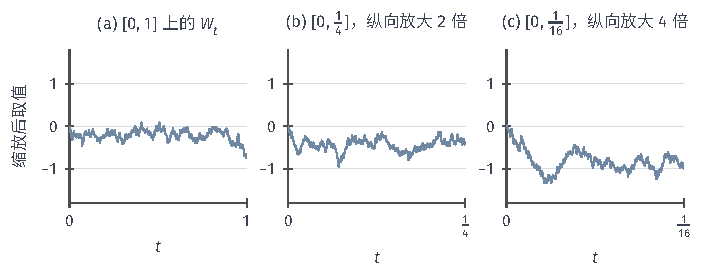
\includegraphics[width=119mm]{figures/03-optimization-evolution-and-signals/02-processes-and-trajectory-evolution/tikz/ctsp-brownian-zoom/figure.pdf}
  \caption{Brownian路径的自相似。用$2^{16}$个独立增量$\mathcal N(0,2^{-16})$累计出一条教学路径（固定随机种子）。(a)$[0,1]$上的整条路径；(b)同一路径在$[0,\frac14]$上的一段，横轴拉伸到$[0,1]$，纵轴乘以$2$；(c)$[0,\frac1{16}]$上的一段，纵轴乘以$4$。按$c^{-1/2}W_{ct}$缩放后，三幅图的起伏幅度相当，放大并没有使路径变得平直。每幅图只绘出约$1100$个网格点。}
  \label{fig:ctsp-brownian-zoom}
\end{figure*}

尺度不变也给出差商的量级。$(W_{t+h}-W_t)/h$服从$\mathcal N(0,1/h)$，标准差$h^{-1/2}$在$h\downarrow0$时发散，所以不能期望在固定时刻存在导数。更强的结论是：以概率一，Brownian路径在任何时刻都不可微。这个结论同时涉及不可数个时刻，不能由逐个固定时刻的计算推出，它的证明见Kallenberg的概率论教材。对后续内容来说，重要的推论是：形如$\mathrm dW_t/\mathrm dt$的“白噪声”不是普通的随机函数，随机微分方程中的$\mathrm dW_t$必须另行解释。

\paragraph{二次变差与总变差}
光滑路径与Brownian路径的差别，可以用两种沿路径的累计量来度量。取$[0,t]$的分割$\pi:0=t_0<t_1<\cdots<t_n=t$，网格宽度$|\pi|=\max_i(t_{i+1}-t_i)$，记$\Delta W_i=W_{t_{i+1}}-W_{t_i}$。考虑平方增量和与绝对增量和
\[
  Q_\pi=\sum_{i}(\Delta W_i)^2,\qquad
  V_\pi=\sum_i|\Delta W_i| .
\]

\begin{theorem}[Brownian运动的二次变差]
  \label{thm:ctsp-brownian-qv}
  对$[0,t]$上任意一列网格宽度趋于零的确定分割$\pi_n$，$Q_{\pi_n}\to t$在$L^2$中成立，从而依概率成立。
\end{theorem}

\begin{proof}
增量独立且$\Delta W_i\sim\mathcal N(0,\Delta t_i)$，所以$\mathbb EQ_\pi=\sum_i\Delta t_i=t$。由正态四阶矩$\mathbb E(\Delta W_i)^4=3(\Delta t_i)^2$，$\operatorname{Var}((\Delta W_i)^2)=2(\Delta t_i)^2$，再由独立性
\[
  \mathbb E(Q_\pi-t)^2=\operatorname{Var}(Q_\pi)=2\sum_i(\Delta t_i)^2\leq2t|\pi| .
\]
网格宽度趋零时右端趋零。
\end{proof}

网格加细时平方增量和的极限称为\term{二次变差}（quadratic variation），记作$[W]_t$；定理说明$[W]_t=t$。二次变差与方差回答的问题不同。方差$\operatorname{Var}(W_t)=t$是在固定时刻对大量实现求平均；二次变差是在一条实现上沿时间累计平方增量，再加细分割。两者在这里数值相同，是Brownian增量方差与时间长度成正比的结果。

绝对增量和的行为完全相反。对等分分割，$\mathbb E|\Delta W_i|=\sqrt{2\Delta t_i/\pi}$，所以$\mathbb EV_\pi=\sqrt{2nt/\pi}\to\infty$。更进一步，路径在每个区间上几乎必然具有无限\term{总变差}（total variation），即所有分割上$V_\pi$的上确界为无穷。理由是：若某条连续路径$x$在$[0,t]$上总变差有限，则
\[
  \sum_i(\Delta x_i)^2\leq\max_i|\Delta x_i|\cdot\sum_i|\Delta x_i|\longrightarrow0,
\]
因为连续函数在紧区间上一致连续，$\max_i|\Delta x_i|\to0$。而定理~\ref{thm:ctsp-brownian-qv}说明，沿一列分割$Q_{\pi_n}\to t$依概率成立，取一个子列便几乎必然收敛到$t>0$。两者矛盾，所以有限总变差的路径只构成零概率集合。对所有有理端点区间取可数并，结论对所有区间同时成立。

图~\ref{fig:ctsp-quadratic-variation}沿二进分割比较了这两个累计量。Brownian路径的平方增量和停在$1$附近，绝对增量和则按$\sqrt n$增长；光滑路径$\sin(2\pi t)$恰好相反，平方增量和趋零，绝对增量和趋于有限的总变差$4$。

\begin{figure}[htbp]
  \centering
  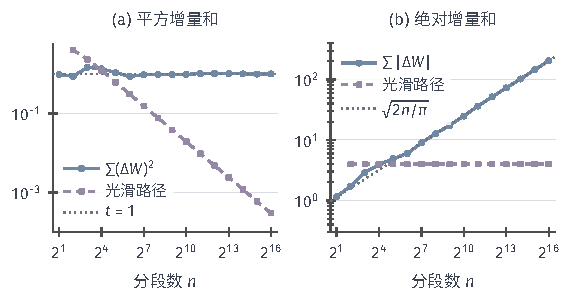
\includegraphics[width=97mm]{figures/03-optimization-evolution-and-signals/02-processes-and-trajectory-evolution/tikz/ctsp-quadratic-variation/figure.pdf}
  \caption{同一条Brownian教学路径（$2^{16}$个独立增量，固定随机种子）与光滑路径$\sin(2\pi t)$在$[0,1]$上沿二进分割的累计量，双轴均为对数刻度。(a)平方增量和：Brownian路径趋近二次变差$1$，光滑路径按$1/n$趋零；(b)绝对增量和：Brownian路径沿参考线$\sqrt{2n/\pi}$（期望值）增长，光滑路径趋于总变差$4$。}
  \label{fig:ctsp-quadratic-variation}
\end{figure}

这两条结论共同决定了第~\ref{sec:ctsp-stochastic-integration}节的走向。无限总变差意味着不能把$\int H_t\,\mathrm dW_t$当作逐路径的Stieltjes积分；非零二次变差意味着Taylor展开中的二阶项$\frac12f''(W)(\Delta W)^2$累计后不会消失，普通链式法则需要修正。

\subsection{路径版本与连续时间信息}
\label{sec:ctsp-path-versions}

\paragraph{不可数时刻上的零概率例外}
离散时间中有一条常用的推理：若对每个$n$，事件$\{X_n=Y_n\}$的概率为一，则$\{X_n=Y_n\text{ 对所有 }n\}$的概率也为一，因为可数个零概率集合的并仍是零概率集合。时间连续以后，时刻有不可数多个，这条推理不再成立。

\begin{example}[随机位置的单点尖峰]
  \label{ex:ctsp-single-spike}
  设$\tau\sim\operatorname{Uniform}(0,1)$，令$X_t\equiv0$，$Y_t=\mathbb I\{t=\tau\}$，$t\in[0,1]$。对每个固定的$t$，$\mathbb P(X_t\neq Y_t)=\mathbb P(\tau=t)=0$，所以两个过程的有限维分布完全相同。但对每个结果$\omega$，$Y$的路径都在$\tau(\omega)$处取值$1$，于是$\mathbb P(X_t=Y_t\text{ 对所有 }t)=0$。$X$的路径连续，$Y$的路径处处不连续于$\tau$。
\end{example}

图~\ref{fig:ctsp-path-versions}画出了一次实现。有限维分布无法区分两者，所以“Brownian运动的路径是否连续”不是有限维分布能回答的问题，只能在同分布的版本中挑出路径性质合适的那一个。

\begin{figure}[htbp]
  \centering
  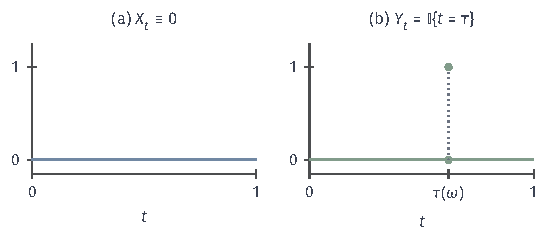
\includegraphics[width=100mm]{figures/03-optimization-evolution-and-signals/02-processes-and-trajectory-evolution/tikz/ctsp-path-versions/figure.pdf}
  \caption{有限维分布相同而路径不同（示例~\ref{ex:ctsp-single-spike}的一次实现，图中取$\tau(\omega)=0.62$）。(a)零路径；(b)只在随机时刻$\tau(\omega)$取$1$的路径，实心点为该时刻的取值，空心点表示路径在那里的左右极限仍为$0$。任一固定时刻恰好落在尖峰上的概率为零。}
  \label{fig:ctsp-path-versions}
\end{figure}

第~\ref{chap:stochastic-processes-and-sample-paths}章区分了两种相等。若对每个$t$，$\mathbb P(X_t=Y_t)=1$，称$Y$是$X$的修改；若存在一个概率为一的事件，在其上$X_t=Y_t$对所有$t$同时成立，称两者不可区分。示例中的$Y$是$X$的修改，却与$X$可以区分。路径正则性正好弥补二者之间的缺口。

\begin{lemma}[右连续修改不可区分]
  \label{lem:ctsp-right-continuous-modification}
  若$X$与$Y$互为修改，且两者的路径几乎必然右连续，则$X$与$Y$不可区分。
\end{lemma}

\begin{proof}
令$D=\mathbb Q\cap[0,\infty)$。$D$可数，所以$\mathbb P(X_q=Y_q\text{ 对所有 }q\in D)=1$。对任意$t$取$q_n\in D$，$q_n\downarrow t$，在上述事件与两条路径都右连续的事件之交上，$X_t=\lim X_{q_n}=\lim Y_{q_n}=Y_t$。
\end{proof}

本章的过程都取\term{右连续有左极限}（càdlàg）的版本：每条路径在每个时刻右连续，并且左极限存在。Poisson过程和以后的跳跃过程天然如此，Brownian运动和连续Itô过程则是其中路径连续的特例。引理~\ref{lem:ctsp-right-continuous-modification}保证这样的版本若存在，则在不可区分的意义下唯一。

\paragraph{滤过的正则条件}
信息结构也需要同样的补充。离散时间中，滤过只需逐个时刻递增；连续时间中还要求它在两种意义下“没有缺口”。一是完备：$\mathcal F_0$包含所有概率零集合的子集，这样在零概率集合上修改一个适应过程后仍然适应。二是右连续：$\mathcal F_t=\bigcap_{s>t}\mathcal F_s$，即“在$t$之后任意短时间内就能知道的事”在$t$时已经知道。同时满足两者时称滤过满足\term{通常条件}（usual conditions）。

右连续性的用途在停时中最清楚。设$X$连续适应，$G$是开集，考虑首次进入时刻$\tau=\inf\{t:X_t\in G\}$。在时刻$t$判断“$\tau<t$”只需看$t$之前的有理时刻，所以$\{\tau<t\}\in\mathcal F_t$；判断“$\tau\leq t$”却可能需要看$t$之后一瞬间路径是否进入$G$。右连续滤过使$\{\tau\leq t\}=\bigcap_n\{\tau<t+1/n\}\in\bigcap_n\mathcal F_{t+1/n}=\mathcal F_t$。Brownian运动的自然滤过经过完备化后满足通常条件，Poisson过程亦然\scite{math-kallenberg2021probability}。本章此后默认滤过满足通常条件。

\paragraph{联合可测与可预测}
随时间积分还需要一种联合可测性。积分$\int_0^tX_s\,\mathrm ds$同时用到时间变量与随机结果；即使每个$X_s$都$\mathcal F_s$可测，若$(s,\omega)\mapsto X_s(\omega)$不是联合可测的，积分甚至可能不是随机变量。若对每个$t$，映射$(s,\omega)\mapsto X_s(\omega)$在$[0,t]\times\Omega$上对$\mathcal B([0,t])\otimes\mathcal F_t$可测，称$X$\term{渐进可测}（progressively measurable）。渐进可测保证$\int_0^tX_s\,\mathrm ds$是$\mathcal F_t$可测的，也保证停时处的取值$X_\tau$可测。

右连续适应过程都是渐进可测的。固定$t$，令$X^{(n)}_s=X_{\min\{(k+1)t/2^n,t\}}$，$s\in[kt/2^n,(k+1)t/2^n)$。每个$X^{(n)}$在$[0,t]\times\Omega$上只取有限个$\mathcal F_t$可测的值，对乘积$\sigma$代数可测；右连续性使$X^{(n)}_s\to X_s$逐点成立，极限保持可测性。左连续适应过程同理。

另一种要求来自事件发生的先后。计数路径在到达时刻$T_k$跳跃，跳后的值$N_{T_k}$在跳跃前不可能知道；如果一个系数要在“事件发生前”就确定，它只能使用严格早于当前时刻的信息。由全部左连续适应过程生成的$\sigma$代数称为可预测$\sigma$代数，对它可测的过程称为\term{可预测过程}。它也由形如$(s,u]\times A$、$A\in\mathcal F_s$的矩形生成：在$s$时刻已知事件$A$是否发生，便可决定在$(s,u]$上取什么值。连续适应过程和左极限过程$N_{t-}$都是可预测的，跳后的$N_t$则不是。第~\ref{sec:ctsp-time-jump-integrals}节将说明这一区别怎样决定跳跃积分的均值。

\paragraph{连续时间的停时}
第~\ref{chap:stochastic-processes-and-sample-paths}章与第~\ref{chap:discrete-time-stochastic-processes}章在离散时间中用“每一步都能判断是否已经停止”刻画停时。连续时间把这一要求放到每个实数时刻上。

\begin{definition}[连续时间停时]
  \label{def:ctsp-stopping-time}
  取值于$[0,\infty]$的随机变量$\tau$称为相对于$(\mathcal F_t)$的\term{停时}，若对每个实数$t\geq0$，$\{\tau\leq t\}\in\mathcal F_t$。与之相伴的信息为$\mathcal F_\tau=\{A\in\mathcal F:A\cap\{\tau\leq t\}\in\mathcal F_t\text{ 对所有 }t\geq0\}$。
\end{definition}

下面三个例子分别检查定义所需的适应性、路径正则性与目标集合条件。

第一，连续适应过程首次到达闭集$F$的时刻$\tau_F=\inf\{t:X_t\in F\}$是停时。记$d(x,F)$为点到$F$的距离。由路径连续和$F$闭，$\tau_F\leq t$当且仅当$\inf_{s\in[0,t]}d(X_s,F)=0$；连续性又允许把下确界只取在可数集$(\mathbb Q\cap[0,t])\cup\{t\}$上，因此该事件属于$\mathcal F_t$。若改用跳跃路径，或把闭集换成开集，就需要右连续滤过等额外条件。

第二，Poisson过程的第$k$次到达时刻是停时，因为$\{T_k\leq t\}=\{N_t\geq k\}\in\mathcal F_t$。跳跃路径的事件时刻可以由当前计数判断，不需要路径连续。

第三，作为反例，令$\sigma=\sup\{t\leq1:W_t=0\}$为Brownian运动在$[0,1]$上最后一次回到零的时刻。判断$\sigma\leq t$需要知道$t$之后到$1$为止路径是否再回到零，这依赖未来，所以$\sigma$不是停时。

连续停时可以取不可数多个值，这使离散时间中“按停时取值分解再求和”的证明无法直接使用。下面的离散化从上方逼近停时，是本章反复使用的桥梁：令
\begin{equation}
  \tau_n=\frac{\lfloor2^n\tau\rfloor+1}{2^n}\quad(\tau<\infty),\qquad\tau_n=\infty\quad(\tau=\infty).
  \label{eq:ctsp-dyadic-stopping}
\end{equation}
每个$\tau_n$只取可数多个二进值，并且$\tau_n\downarrow\tau$。它仍是停时：$\tau_n\leq t$等价于$\tau<\lfloor2^nt\rfloor/2^n$，后者属于$\mathcal F_{\lfloor2^nt\rfloor/2^n}\subseteq\mathcal F_t$。从上方逼近是必要的，向下取整得到的随机时刻需要“提前知道”停止，一般不是停时。停止后的Markov规律与鞅期望将分别在第~\ref{sec:ctsp-strong-markov}节和第~\ref{sec:ctsp-optional-sampling}节借助这一逼近建立。
